\documentclass[11pt]{article}

\usepackage{hyperref}  % links
\usepackage{graphicx}  % images
\usepackage{listings}  % code
\usepackage{authblk}  % author info
\usepackage{biblatex}  % bibliography

\addbibresource{bib.bib}

% Preamble
\title{Angular, React or Vue.js: Which is Most Practical?}
\author{Brent Schaeffer}
\date{\today}

% Document body

\begin{document}

\maketitle

\begin{abstract}
    This paper takes a more in dpeth look into three popular JavaScript based web frameworks that are common into today's industry
\end{abstract}


Before getting into the deeper parts of web frameworks, specifically the ones we will be
exploring: Angular, React and Vue.js, we must understand the basics of what is a web framework,
how are they used, and what purpose do they serve in today's world of programming. 
A majority of modern websites use JavaScript in some shape or form, to make the pages more
interactive and to handle functionality(Saks, Elar). Traditionally in the past webpages were large multi-page applications (MPAs)
that had to load different HTML documents whenever a user chagned pages or requested new content from the server.
This however is a relatively slow and time consuming option compared to the modern day idea a of single page application
(SPA). SPAs work in improving the time it takes to load an application by fetching the data from a server, 
then updating the current page contents with the fetched data, instead of loading a whole new document. 
This in turn also increases the quality of the users experience with the applications interface. Now this does not mean
that MPAs are not used they are, but working with web frameworks allows the reduction of how many documents that are 
needed for that application. In other terms frameworks are designed to support and help developers develop web applications
in a more consistent and reliable way, as said by Elar Saks, "Frameworks dictate the application development workflow, reduce the development time and
possible errors". In the world of frameworks there are tons of available choices and the criteria to be considered one is somewhat open and can at times
be confused with libraries. A library generally consists of pre-written code, classes, procedures, scripts, configuration data, and more.
Mostly, it can be integrated in an existing project with ease and used to shorten development time. This is due to the fact that many 
issues concerning basic algorithms and functions have already been solved by another expert programmer in the community(Wohlgethan, Eric).
It can be thought of in this manner, libraries are used to enhance a program or application, but on their own they cannot offer a complete 
stack of tools for development purposes. A simplified idea of this can be seen below in figure \ref{fig:1}.In comparison to libraries, 
frameworks indeed offer a complete stack of helpful functions and take responsibility for decisions that otherwise the developer
would have to make prior to actually writing the application’s code. This includes strategies for in-app routing of URL paths, 
state management, bundling and others. Furthermore, frameworks provide workflow improvements which include best practices
for basic development aspects like the overall structure of an application or generating boilerplate code. In a sense one can think of
frameworks as fully fledged libraries while there also exists other libraries that contain useful tools, but are not a complete 
set of tools to stand on their own. 

\begin{figure}[h]
    \centering
    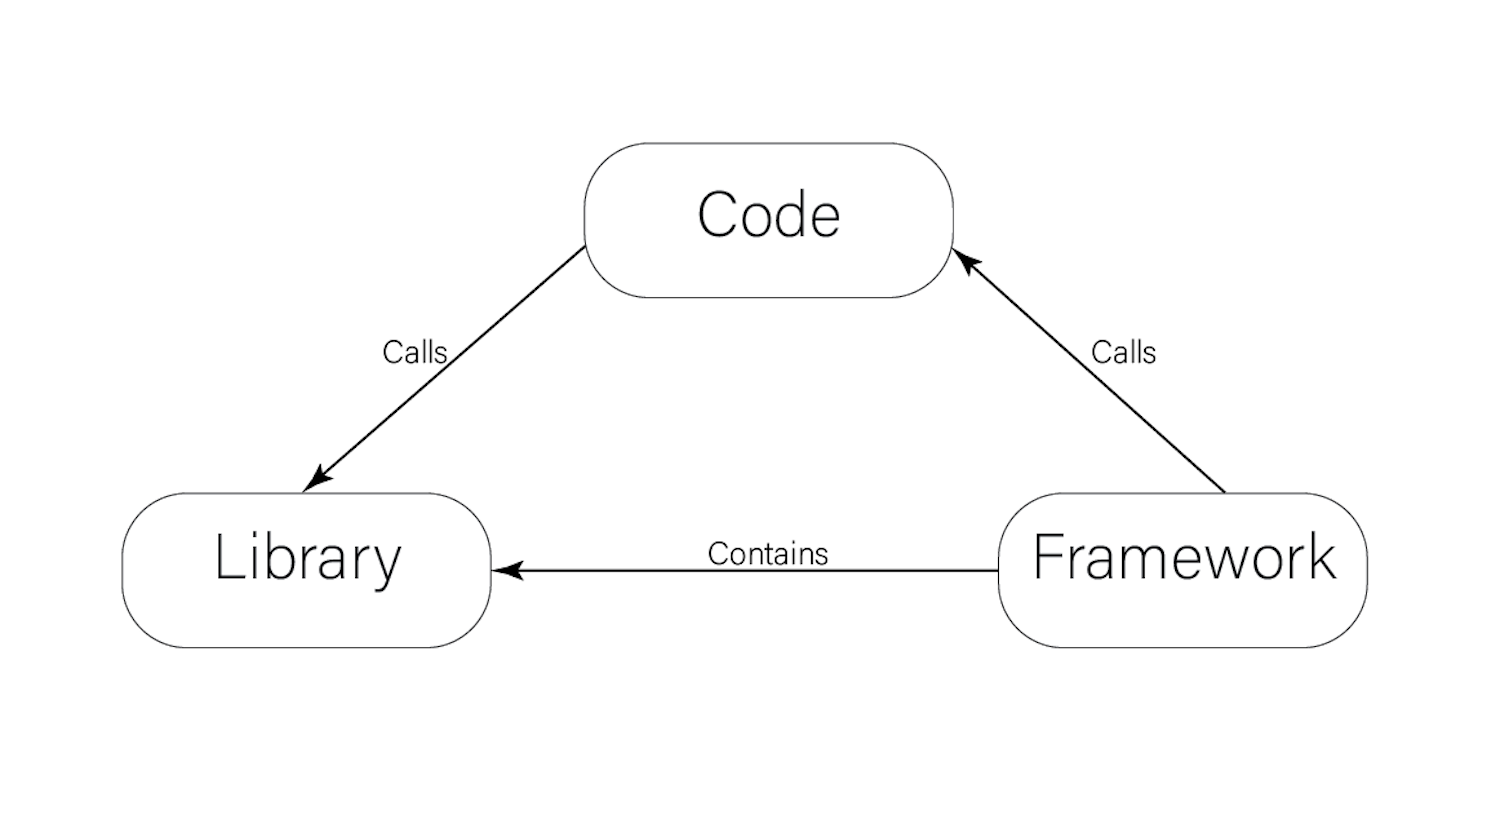
\includegraphics{flowchart}
    \caption{Libraries compared to frameworks}
    \label{fig:1}
\end{figure}


\end{document}